\chapter{Roboternavigation im Kraftfeld}

Die Roboternavigation der Potenzialfeldmethode entspricht der Bewegung eines Körpers im \textit{Gravitationsfeld} des Potenzialfelds.

\section{Berechnung der Gradienten}

Das Gravitationsfeld entspricht dem Gradientenfeld des Potenzialfelds: Auf jede Koordinate im Gravitationsfeld wirkt Gravitationskraft zerlegt in die drei kartesische Komponenten des Konfigurationsraums. Jedes dieser drei Kraftfelder $F_{x/y/rotation}(\texttt{x}, \texttt{y}, \texttt{rotation})$ gibt für die jeweilige Dimension des Konfigurationsraums die Größe der Gravitationskraft in der Koordinate (\texttt{x}, \texttt{y}, \texttt{rotation}) an:
\begin{equation*}
 F_{x}(\texttt{x}, \texttt{y}, \texttt{rotation}), F_{y}(\texttt{x}, \texttt{y}, \texttt{rotation}), F_{rotation}(\texttt{x}, \texttt{y}, \texttt{rotation}) = -\nabla U(\texttt{x}, \texttt{y}, \texttt{rotation})
\end{equation*}

Um die Gradienten zwischen dem letzten Rotationsschritt und $0$° zu berechnen, wird die erste und letzte Rotationsebene an das jeweils andere Ende der Dimension \texttt{potential[rotation]} kopiert.
\begin{equation*}
\hspace*{-0.0075\linewidth}
\resizebox{1.05\linewidth}{!}{
$
	\texttt{potential\_padded} = \texttt{np.concatenate([potential[0], potential, potential[\texttt{rotations - 1}]])}
$
}
\hspace*{-0.0075\linewidth}
\end{equation*}

Die kopierten Rotationsebenen werden nach Berechnung der Kraftfelder entfernt:
\begin{equation*}
\hspace*{-0.075\linewidth}
\resizebox{1.15\linewidth}{!}{
$
\texttt{force\_field\_rotation}, \texttt{ force\_field\_y}, \texttt{ force\_field\_x} = -\texttt{np.gradients(potential\_padded)[1:rotation-1]}
$
}
\hspace*{-0.075\linewidth}
\end{equation*}

Somit entsprechen Gradienten $ \texttt{force\_field\_rotation[rotation]} > 0 $ einer Kraft in Richtung $\texttt{force\_field\_rotation[0]}$ und Gradienten $ \texttt{force\_field\_rotation[0]} < 0 $ einer Kraft in Richtung $\texttt{force\_field\_rotation[rotation]}$.

\begin{figure}[h!]
	\centering
	\footnotesize
	\centerline{\resizebox{0.45\linewidth}{!}{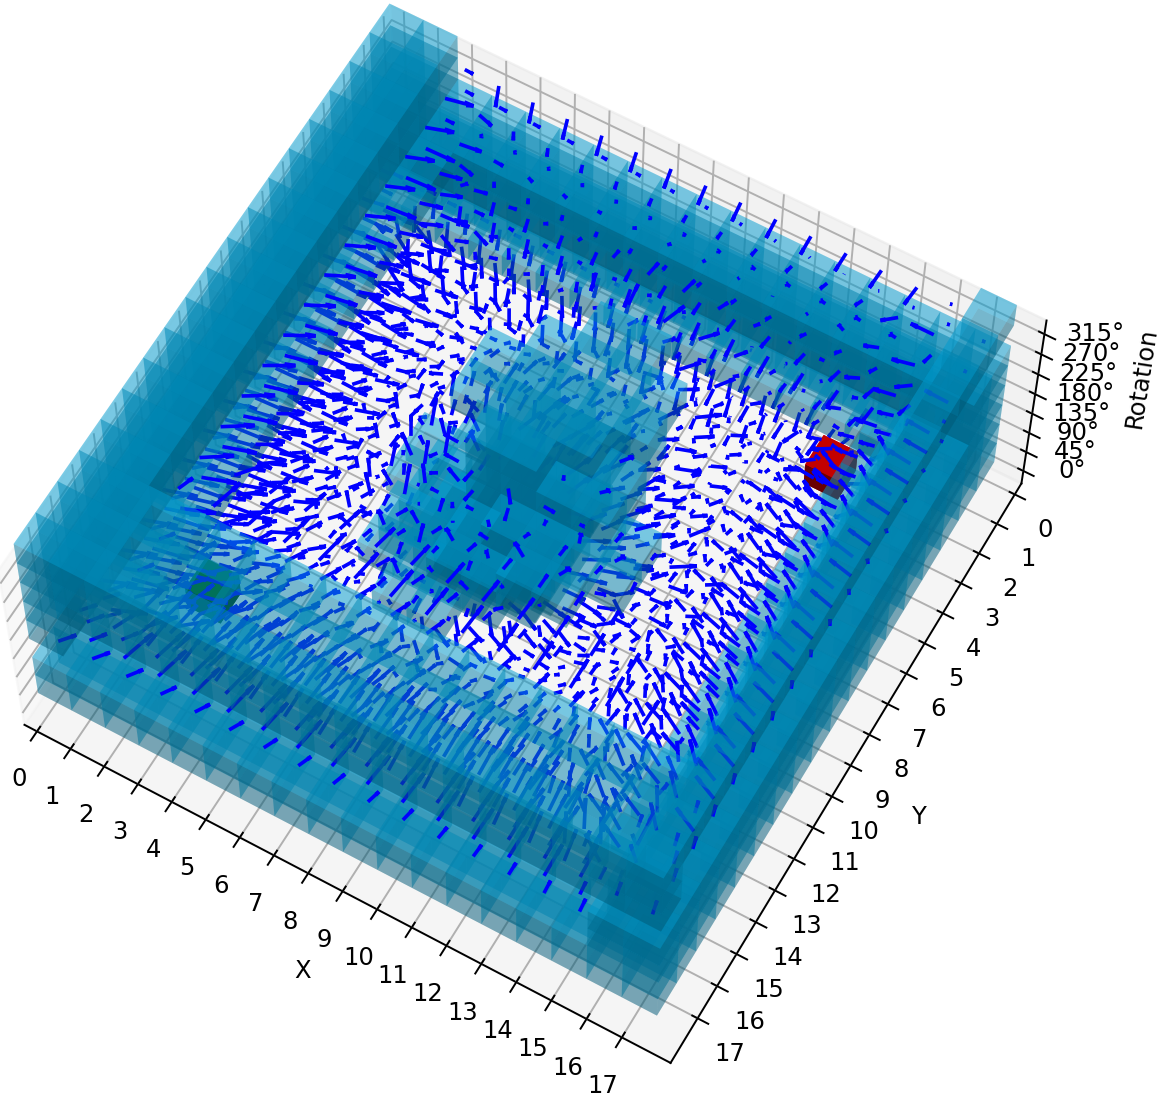
\includegraphics{bilder/force-field.png}}}
	\caption{Darstellung des Gradientenfelds als Kraftpfeile im Konfigurationsraum.}
\end{figure}

\subsection{Gradienten an Grenzen und Hindernissen}

Um die Grenzen des Konfigurationsraums einzuhalten, werden unzulässige Gradienten an den $X$- und $Y$-Grenzen auf $0$ gesetzt. Durch dieses manuelle Abschneiden der Kräfte können an den Grenzen lokale Minima entstehen.
\begin{figure}[h!]
	\centering
	\footnotesize
	\centerline{\resizebox{0.65\linewidth}{!}{\input{bilder/gradient-clipping_latex.pdf_tex}}}
	\caption{Das Setzen der Gradienten in Grenznähe auf 0 kann zu lokalen Minima führen.}
\end{figure}
Im Potenzialfeld \texttt{potential} haben Hindernisse das Potenzial \texttt{np.nan}. Somit berechnet \texttt{np.gradients()} für jede an ein Hindernis grenzende Koordinate den Gradienten \texttt{np.nan}.
Stattdessen sollen Hindernisse bei Berechnung der Gradienten wie Grenzen des Konfigurationsraums interpretiert werden. Ebenso wird hier die Kraft der jeweiligen Dimension auf 0 gesetzt, sollte negative Gradient in Richtung des Hindernisses zeigen. Nachfolgende Tabelle zeigt dies beispielhaft für Hindernisse im Kraftfeld der $X$-Achse \texttt{force\_field\_x} gezeigt:
\begin{table}[H]
\centerline{\resizebox{0.9\linewidth}{!}{
\begin{tabular}{|c|c|c|}
\hline
\textbf{Koordinate Hindernis}                                                & \textbf{\texttt{force\_field\_x[rotation][y][x] = -1*...}}                                                        & \textbf{\texttt{= 0}, wenn ...} \\ \hline
$x+1$ (rechts)                                                               & $\texttt{potential[z, y, x]} - \texttt{potential[z, y, x-1]}$ & $>0$                               \\ \hline
$x-1$ (links)                                                                & $\texttt{potential[z, y, x+1]} - \texttt{potential[z, y, x]}$ & $<0$                                \\ \hline
\begin{tabular}[c]{@{}c@{}}$x+1$ und $x-1$\\ (rechts und links)\end{tabular} & \texttt{0}                                                                           & N/A                                 \\ \hline
\end{tabular}}}
\end{table}
Wird die Kraft einer Dimension auf $0$ gesetzt, wobei die Kräfte der anderen Kraftfelder an dieser Koordinate ebenfalls $0$ sind, entsteht ein lokales Minimum oder Plateau.

\subsection{Behandlung lokaler Maxima}

Im Unterschied zu einem lokalen Minimum oder Plateau ist bei einem lokalen Maximum das Potenzial der Nachbarn streng monoton niedriger als das der aktuellen Koordinate.
In diesen Fällen wird zu einem der Nachbarn eine künstliches Hindernis gesetzt und der Gradient neu berechnet.
\begin{figure}[H]
	\centering
	\footnotesize
	\centerline{\resizebox{0.9\linewidth}{!}{\input{bilder/local-maxima_latex.pdf_tex}}}
	\caption{Lokale Maxima können durch künstliche Hindernisse behoben werden.}
\end{figure}


\section{Gradientenabstieg}

Die berechneten Gradientenfelder ermöglichen die Roboternavigation durch das \textit{Gradientenabstiegsverfahren}:

Pro Verarbeitungsschritt wird für eine Koordinate $(\texttt{x},\texttt{x},\texttt{rotation})$ die nächste Koordinate basierend auf der beträgsmäßig größten Gravitationskraft in $F_{x}(\texttt{x}, \texttt{y}, \texttt{rotation})$, $F_{y}(\texttt{x}, \texttt{y}, \texttt{rotation})$ und $F_{rotation}(\texttt{x}, \texttt{y}, \texttt{rotation})$ gewählt, bis in einer Koordinate ein Kräftegleichgewicht $F_{x}(\texttt{x}, \texttt{y}, \texttt{rotation}) = F_{y}(\texttt{x}, \texttt{y}, \texttt{rotation}) = F_{rotation}(\texttt{x}, \texttt{y}, \texttt{rotation}) = 0$ herrscht:


\begin{algorithm}
\caption{Gradientenabstiegsverfahren}
\begin{algorithmic}[1]
    \State \textbf{Initialisierung:}
    \State \hspace{\algorithmicindent} $(\texttt{x}_{\text{current}}, \texttt{y}_{\text{current}}, \texttt{rotation}_{\text{current}}) = \texttt{start\_point}$
    \State \hspace{\algorithmicindent} Visited $V \leftarrow \emptyset$
	\vspace*{0.3cm}
    \While{true}
		\vspace*{0.1cm}
        \If{$(\texttt{x}_{\text{current}}, \texttt{y}_{\text{current}}, \texttt{rotation}_{\text{current}}) = \texttt{goal\_point}$}
            \State \textbf{return} Ziel gefunden
        \EndIf
		\vspace*{0.1cm}
        \State $\texttt{force\_field\_x/y/rotation}\texttt{[}\texttt{rotation}_{\text{current}}\texttt{][}\texttt{y}_{\text{current}}\texttt{][}\texttt{x}_{\text{current}}\texttt{]} = 0$
        \State $(\texttt{dx}, \texttt{dy}, \texttt{drotation}) \gets \max(|\texttt{force\_field\_x/y/rotation}\texttt{[}\texttt{rotation}_{\text{current}}\texttt{][}\texttt{y}_{\text{current}}\texttt{][}\texttt{x}_{\text{current}}\texttt{]}|)$
		\vspace*{-0.3cm}
        \If{$(\texttt{dx}, \texttt{dy}, \texttt{drotation}) = (0,0,0)$}
            \State \textbf{return} Lokales Minimum oder Plateau
        \EndIf
     	\vspace*{0.1cm}
        \State $(\texttt{x}_{\text{current}}, \texttt{y}_{\text{current}}, \texttt{rotation}_{\text{current}}) \gets (\texttt{x}_{\text{current}} + \texttt{dx}, \texttt{y}_{\text{current}} + \texttt{dy}, \texttt{rotation}_{\text{current}} + \texttt{drotation})$
		\vspace*{-0.3cm}
        \If{$(\texttt{x}_{\text{current}}, \texttt{y}_{\text{current}}, \texttt{rotation}_{\text{current}}) \in V$}
            \State \textbf{return} Lokales Minimum
		\Else
			\State $(\texttt{x}_{\text{current}}, \texttt{y}_{\text{current}}, \texttt{rotation}_{\text{current}}) \rightarrow V$
        \EndIf
		\vspace*{0.1cm}
    \EndWhile
\end{algorithmic}
\end{algorithm}

Der Gradientenabstieg muss dabei für die erlaubten Translationen des Konfigurationsraums diskretisiert werden: 
Gemäß der definierten Roboterbewegungen in Kapitel X (TODO!) darf der Roboter pro Verarbeitungsschritt nur eine Translation um eine Einheit entlang der Dimensionen \texttt{[rotation][y][x]} durchführen. Somit gilt:
\begin{equation*}
(\texttt{dx}, \texttt{dy}, \texttt{drotation}) \in \{(1,0,0)(-1,0,0),(0,1,0),(0,-1,0),(0,0,1),(0,0,-1)\}
\end{equation*}






